
\section{Лекция 3. Условия Коши-Римана. Голоморфность}
\subsection{Условие Коши-Римана}

\textbfit{Теорема} (Коши-Римана) Пусть $f:U(z_0) \to \mathbb{C}. \ f - \mathbb{C}-$дифференцируема в $z_0 \Leftrightarrow \mathbb{R}-$диф-

ференцируема в $z_0$ и выполнено условие Коши-Римана $\begin{cases}
    u_x = v_y \\
    u_y = -v_x
\end{cases}$, т.е. $\frac{\delta f}{\delta \overline{z}}=0$
\[\triangleright (\Rightarrow) f(z_0+\Delta z)-f(z_0)=f'(z_0)\Delta z +\overline{o}(\Delta z) = |f'(z_0)|\left(\begin{array}{ll}
\cos \phi & -\sin \phi \\
\sin \phi & \cos \phi    
\end{array}\right) \left(\begin{array}{ll}
 \Delta x \\
 \Delta y   
\end{array}\right) + \overline{o}(|\Delta z|)\]
\[\Rightarrow u_x = |f'(z_0)|\cdot \cos \phi \ldots \Rightarrow \text{Коши-Римана выполнено, и $f \ \mathbb{R}-$дифференцируема}\]
\[(\Leftarrow) f(z_0+\Delta z)-f(z_0) = \frac{\delta f}{\delta z} \Delta z + \frac{\delta f}{\delta z} \Delta \overline{z}+\overline{o}(\Delta z) = \frac{\delta f}{\delta z}\Delta z + \overline{o}(\Delta z) \Rightarrow\]
\[\Rightarrow f \ \mathbb{C}-\text{дифференцируема и } f'(z_0) = \frac{\delta f}{\delta z}\Big|_{z_0} \blacktriangleleft\]

\textbfit{Пр.} $f(z) = \overline{z} = x-iy$
\[u(x, y) = x, \ v(x, y) = -y\]
\[\begin{cases}
    1 \neq -1 \\
    0 = 0
\end{cases}\]
\[\frac{\delta f}{\delta \overline{z}} = 1 \neq 0\]
\[\text{Условие Коши-Римана не выполнено, значит, не $\mathbb{C}-$дифференцируема.}\]
\textbfit{Опр.} Пусть $\theta \in \mathbb{R}, \ f:U(z_0)\to\mathbb{C}$. Тогда производной по направлению $\theta$ называется $f'_\theta(z_0) = \lim_{\Delta z \to 0, \ \arg \Delta z = \theta} \frac{f(z_0+\Delta z)-f(z_0)}{\Delta z}$
\[f'_0(z_0) = u_x +iv_x\]
\[f'_{\frac{\pi}{2}} = -i(u_y+iv_y)\]
\textbfit{Опр.} Пусть $f-\mathbb{R}-$дифференцируема. Тогда $f-\mathbb{C}-$дифференцируема в $z_0 \Leftrightarrow f'_\theta(z_0)$ не зависит от $\theta$.
\[(\Rightarrow) \text{ очевидно}\]
\[(\Leftarrow) \Delta f = \frac{\delta f}{\delta z}\Delta z. +\frac{\delta f}{\delta \overline{z}}\Delta \overline{z}+\overline{o}(\Delta z) = (1)\]
\[\arg \Delta z = \theta, \ \Delta z = te^{i\theta}\]
\[\Delta \overline{z} = \Delta z e^{-2i\theta}\]
\[(1) = \Delta z \left(\frac{\delta f}{\delta z} + e^{-2i\theta} \frac{\delta f}{\delta \overline{z}}\right)+\overline{o}(\Delta z)=\Delta z f'_\theta (z_0) +\overline{o}(\Delta z)\]
\[\text{Но $f'_\theta$ не зависит от $\theta \Rightarrow f'_0=f''_\frac{\pi}{2}$}\]
\[\frac{\delta f}{\delta z} + \frac{\delta f}{\delta \overline{z}}=\frac{\delta f}{\delta z} -\frac{\delta f}{\delta \overline{z}}\]
\[\Rightarrow \frac{\delta f}{\delta \overline{z}} = 0 \text{, т.е. Коши-Римана.}\]
\textbfit{Пр.} 1) $z=x+iy$
\[\left(\begin{array}{ll}
1 & 0 \\
0 & 1    
\end{array}\right)\]
Условие Коши-Римана выполнено.
\[(z)'=u_x+iv_x=1\]
\[2) \ (z^n)'=nz^{n-1}\]
\[3) \ e^z = e^x(\cos y + i\sin y)\]
\[\left(\begin{array}{ll}
e^x\cos y & -e^x \sin y \\
e^x \sin y & e^x \cos y    
\end{array}\right)\]
Условие Коши-Римана выполнено.
\[(e^z)' = e^x \cos y + ie^x \sin y =e^z\]
\textbfit{Утв.} Пусть $f \in C^1 (U(z_0)), \ f'(z_0) \neq 0, \ f(z_0) = w_0$. Тогда $\exists g: U(w_0)\to U(z_0), g=f^{-1}, g \in C^1(U(w_0)), \ g-\mathbb{C}-$дифференцируема в $w_0$ и $g'(w_0)=\frac{1}{f'(z_0)}$
\[\triangleright f'(z_0) \neq 0 \Rightarrow |f'(z_0)|\neq 0, \ \arg f'(z_0) \text{ определён} ,|J| = |f'(z_0)|\neq 0\]
\[\text{Следовательно, выполнено условие теоремы об обратном отображении. }\]
\[\Rightarrow \exists g : U(w_0)\to U(z_0), \ g \in C^1, \text{ т.е. } \mathbb{R}-\text{дифференцируема и }dg\Big|_{w_0} = (df\Big|_{z_0})^{-1} =\] 
\[\left(|f'(z_0)| \left(\begin{array}{ll}
\cos \phi & -\sin \phi \\
\sin \phi & \cos \phi   
\end{array}\right)\right)^{-1} = \frac{1}{|f'(z_0)|} \left(\begin{array}{ll}
\cos \phi & -\sin \phi \\
\sin \phi & \cos \phi   
\end{array}\right) \text{ т.е. выполнено Коши-Римана}\]
\[g'(w_0) = \frac{1}{f'(z_0)} \blacktriangleleft\]
\textbfit{Пр.} $f(z) = z^2$
\[f'\Big|_{-1} = 2z=-2\]
\begin{center}
    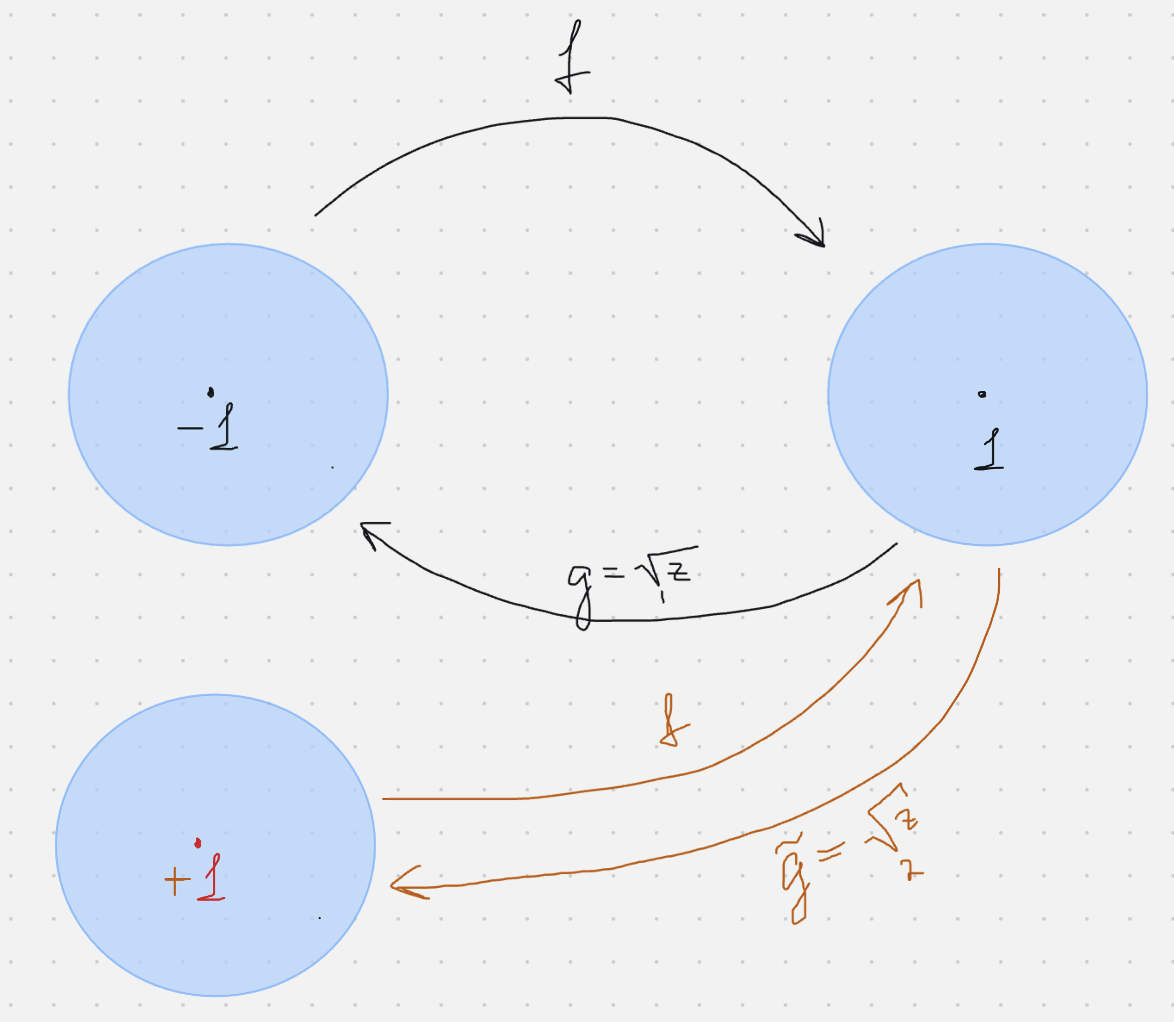
\includegraphics[width=0.5\linewidth]{lection3_1.png}
\end{center}
\[g(1) = \frac{1}{f'(-1)} = -\frac{1}{2} = \frac{1}{2\sqrt{z}_1}\]
\[g(1)=\frac{1}{f'(1)} = \frac{1}{2} = \frac{1}{2\sqrt{z}_2}\]
\textbfit{Пр.} $f(z)=e^z, \ f'(z) =e^z$
\begin{center}
    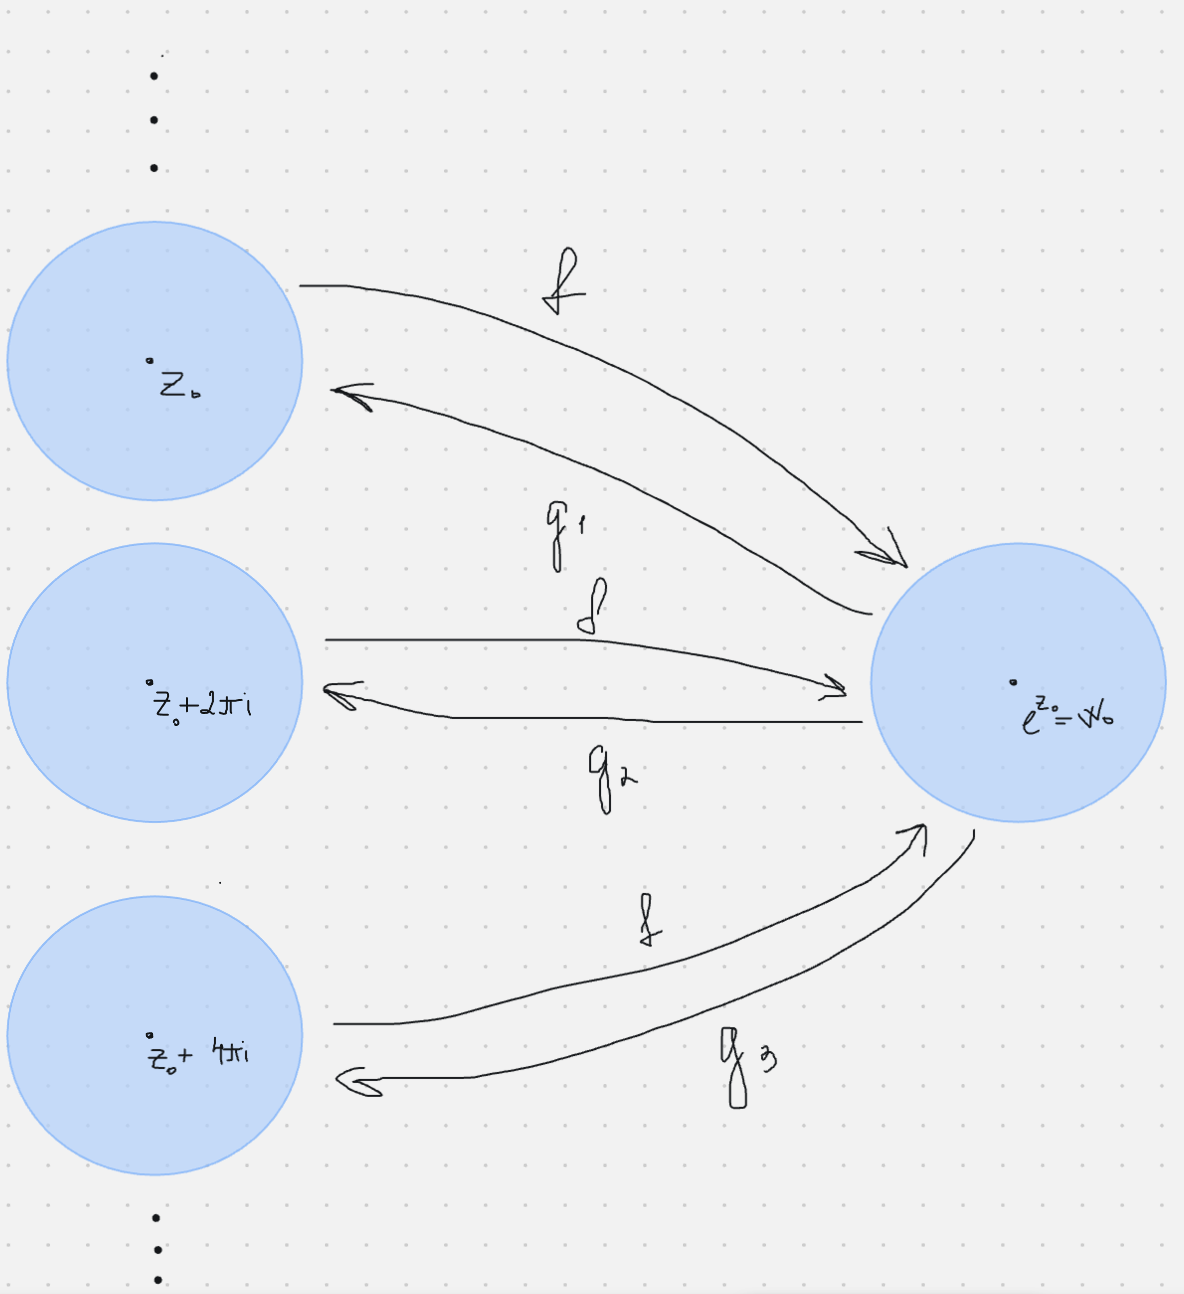
\includegraphics[width=0.5\linewidth]{lection3_2.png}
\end{center}
\[g_1(w_0)=g_1(e^{z_0})=\frac{1}{f'(z_0)}=\frac{1}{e^{z_0}}=\frac{1}{w_0}\]
\[g_i(w_0)=g_1(e^{z_0})=\frac{1}{f'(z_0+2i\pi k)}=\frac{1}{e^{z_0+2i\pi k}}=\frac{1}{w_0}\]

\textbfit{Опр.} Пусть $f: U(z_0)\to \mathbb{C}. \ f$ называется голоморфной в точке $z_0$, если $\exists U_\epsilon(z_0)$, т.ч. $f-\mathbb{C}-$дифференцируема в $U_\epsilon(z_0)$.

Если $f: D \to \mathbb{C}, \ D-$область, то говорят, что $f$ голоморфна в $D$, если она голоморфна в каждой точке $D$. Обозначение $f \in O(D)$

\textbfit{Опр.} Пусть $f:U(\infty)\to \mathbb{C}$. Говорят, что $f \ \mathbb{C}-$ дифференцируема (голоморфна), если $\mathbb{C}-$дифференцируема (голоморфна) в точке $z=0$ функция $F(z) = \begin{cases}
    f(\frac{1}{z}) \\
    f(\infty)
\end{cases}$

\textbfit{Пр.} $f(z) = \begin{cases}
    \frac{1}{z} \\ 0 & z =\infty
\end{cases}$
\[F(z) = \begin{cases}
    z \\ 0 & z = 0
\end{cases}\]

\textbfit{Опр.} Пусть $z_0 \in \overline{\mathbb{C}}, \ f:U(z_0)\to\mathbb{C}, \ f(z_0)=\infty$. Тогда она $\mathbb{C}-$дифференцируема (голоморфна) в $z_0$, если в $z_0$ голоморфна $\frac{1}{z_0}$, т.е. если $f(\infty)=\infty$, то надо изучать $\frac{1}{f(\frac{1}{z})}$ в $z=0$
